\documentclass[aspectratio=169]{beamer}
\usepackage[utf8]{inputenc}
\usepackage{graphicx}
\usepackage{booktabs}
\usepackage{amsmath}
\usepackage{hyperref}

\usepackage{xcolor}
\usetheme{metropolis}
\usecolortheme{default}
\graphicspath{{../../3_Output/Figures/}}

% Footer formatting from Old Deck
\setbeamertemplate{frame footer}{Author Name \hfill Peer-Effects in ESB Adoption \hfill Spring 2026}
\setbeamerfont{page number in head/foot}{size=\tiny}
\definecolor{mDarkTeal}{HTML}{23373b}
\definecolor{mLightBrown}{HTML}{EB811B}
\setbeamercolor{footline}{fg=white, bg=mDarkTeal}

% Title parameters
\title[ESB Peer Effects]{Peer Effects and Electric School Bus Adoption}
\subtitle{Administrative Knowledge Spillovers in Federal Procurement}
\author[Pisharam]{Anirudh Pisharam \\ \textit{Boston College}}
\date{Spring 2026}

\begin{document}

\begin{frame}
    \titlepage
\end{frame}

% -------------------------
% SECTION I: INTRODUCTION
% -------------------------

\begin{frame}{Motivation}
    \begin{itemize}
        \item \textbf{The Transition:} School districts face a massive collective action problem transitioning to electric fleets. 
        \item \textbf{The Observation:} Electric school bus (ESB) adoption is highly clustered geographically.
        \item \textbf{The Core Question:} Does ESB adoption cluster because districts \textit{learn} from one another, or simply because neighbors share similar policies, vendors, and infrastructures?
        \vspace{0.5cm}
        \item Identifying peer effects is notoriously difficult due to the reflection problem and homophily.
    \end{itemize}
\end{frame}

\begin{frame}{Institutional Setting: The EPA Clean School Bus Program}
    \begin{itemize}
        \item \textbf{The Program:} The 2021 Bipartisan Infrastructure Law authorized \$5 billion over five years for the EPA Clean School Bus (CSB) Program.
        \item \textbf{The Mechanism:} Round 1 (FY 2022) distributed almost \$1 \textbf{billion via a randomized lottery} system.
        \item \textbf{The Natural Experiment:} This lottery generates conditionally exogenous shocks to specific localized networks, breaking the reflection problem. 
    \end{itemize}
\end{frame}

\begin{frame}{Current Results (Work in Progress)}
    \begin{enumerate}
        \item \textbf{Peer Effects Exist:} An exogenous increase in an adopted neighbor yields a $\sim 0.75$ percentage point increase in own focal adoption likelihood (relative to a $\sim 10.4\%$ baseline adoption rate).
        \item \textbf{Mechanism -- Administrative Spillovers:} Suggestive evidence implies the effect unfolds through grant-writing networks (applications) rather than physical salience (seeing a bus).
        \item \textbf{Deep Localization:} The effect decays monotonically as spatial radius expands from 15 to 60 miles.
    \end{enumerate}
\end{frame}

% -------------------------
% SECTION II: DATA
% -------------------------

\begin{frame}{Data and Sample Construction}
    \begin{itemize}
        \item \textbf{Universe:} 19,495 public school districts across the contiguous United States.
        \item \textbf{Geometry \& Network Restrictions:} Drop non-contiguous, unmatched, charter, and private schools due to distinct procurement and overlapping boundaries (leaves 13,075 districts).
        \item \textbf{At-Risk Panel:} Construct a discrete-time district-year panel (2020-2024), where districts exit the risk set once they adopt. We explicitly drop focal R1 winners to isolate \textit{peer} effects, leaving a final estimation sample of 12,694 districts.
        \item \textbf{Final Panel Size:} 86,960 district-year observations.
        \item \textbf{Adoption Rate Measurement:} The WRI database tracks committed ESBs; while some precise quarter-level stage dates are manually documented, others are estimated using WRI's standard imputation procedure when public announcements lack exact dates.
    \end{itemize}
\end{frame}

\begin{frame}{Defining the Variables \& Network}
    \begin{itemize}
        \item \textbf{Measuring Outcomes (The Timing Difference):}
        \begin{itemize}
            \item \textit{Awarded Year:} Date district was notified of funding limit (Main Outcomes).
            \item \textit{Operational Year:} Physical date buses actually hit the road (Mechanism Test).
        \end{itemize}
        \vspace{0.2cm}
        \item \textbf{Constructing the Sub-Networks (Spatial Weights):}
        \begin{itemize}
            \item Primary Strategy: $K=6$ nearest geographic public school districts.
            \item Robustness tests utilizing absolute distance radii (15, 30, and 60 miles) maps.
            \item \textit{Note: Charter schools are currently excluded due to overlapping spatial boundaries and distinct procurement models (planned for future distance-based robustness).}
        \end{itemize}
        \vspace{0.2cm}
        \item \textbf{The Endogenous Variable \& Instrument:}
        \begin{itemize}
            \item \textit{Peer Stock ($P_{i,t-1}$):} Cumulative count of neighbors previously awarded ESBs.
            \item \textit{Instrument ($Z_i^{R1}$):} Number of neighbors randomly awarded in EPA R1.
        \end{itemize}
    \end{itemize}
\end{frame}

\begin{frame}[label=summary_balance]{Summary Statistics \& Balance}
    \begin{itemize}
        \item \textbf{Summary Statistics:} Our primary sampling frame of 19,495 districts captures the near-universe of public school districts, allowing us to describe both early-adopters and non-adopters on key demographics.
        \vspace{0.1cm}
        \hyperlink{app_summary}{\textbf{\color{mLightBrown} $\rightarrow$ See Sample Descriptives}}
        \vspace{0.2cm}
        \item \textbf{Balance Profile (Instrument Validity):} Since our spatial shock relies on randomized neighbor lottery outcomes, we first validate the underlying EPA lottery. 
        \item \textbf{Key Insight:} Within the priority strata applicant pool, R1 Winners and R1 Losers are essentially perfectly balanced on pre-2022 observables (e.g., prior PM2.5, student enrollment, poverty rates). This confirms the instrument provides exogenous variation.
        \vspace{0.1cm}
        \hyperlink{app_balance}{\textbf{\color{mLightBrown} $\rightarrow$ See Balance Tests}}
    \end{itemize}
\end{frame}

\begin{frame}{Spatial Clustering of ESB Adoption (National Scale)}
    \centering
    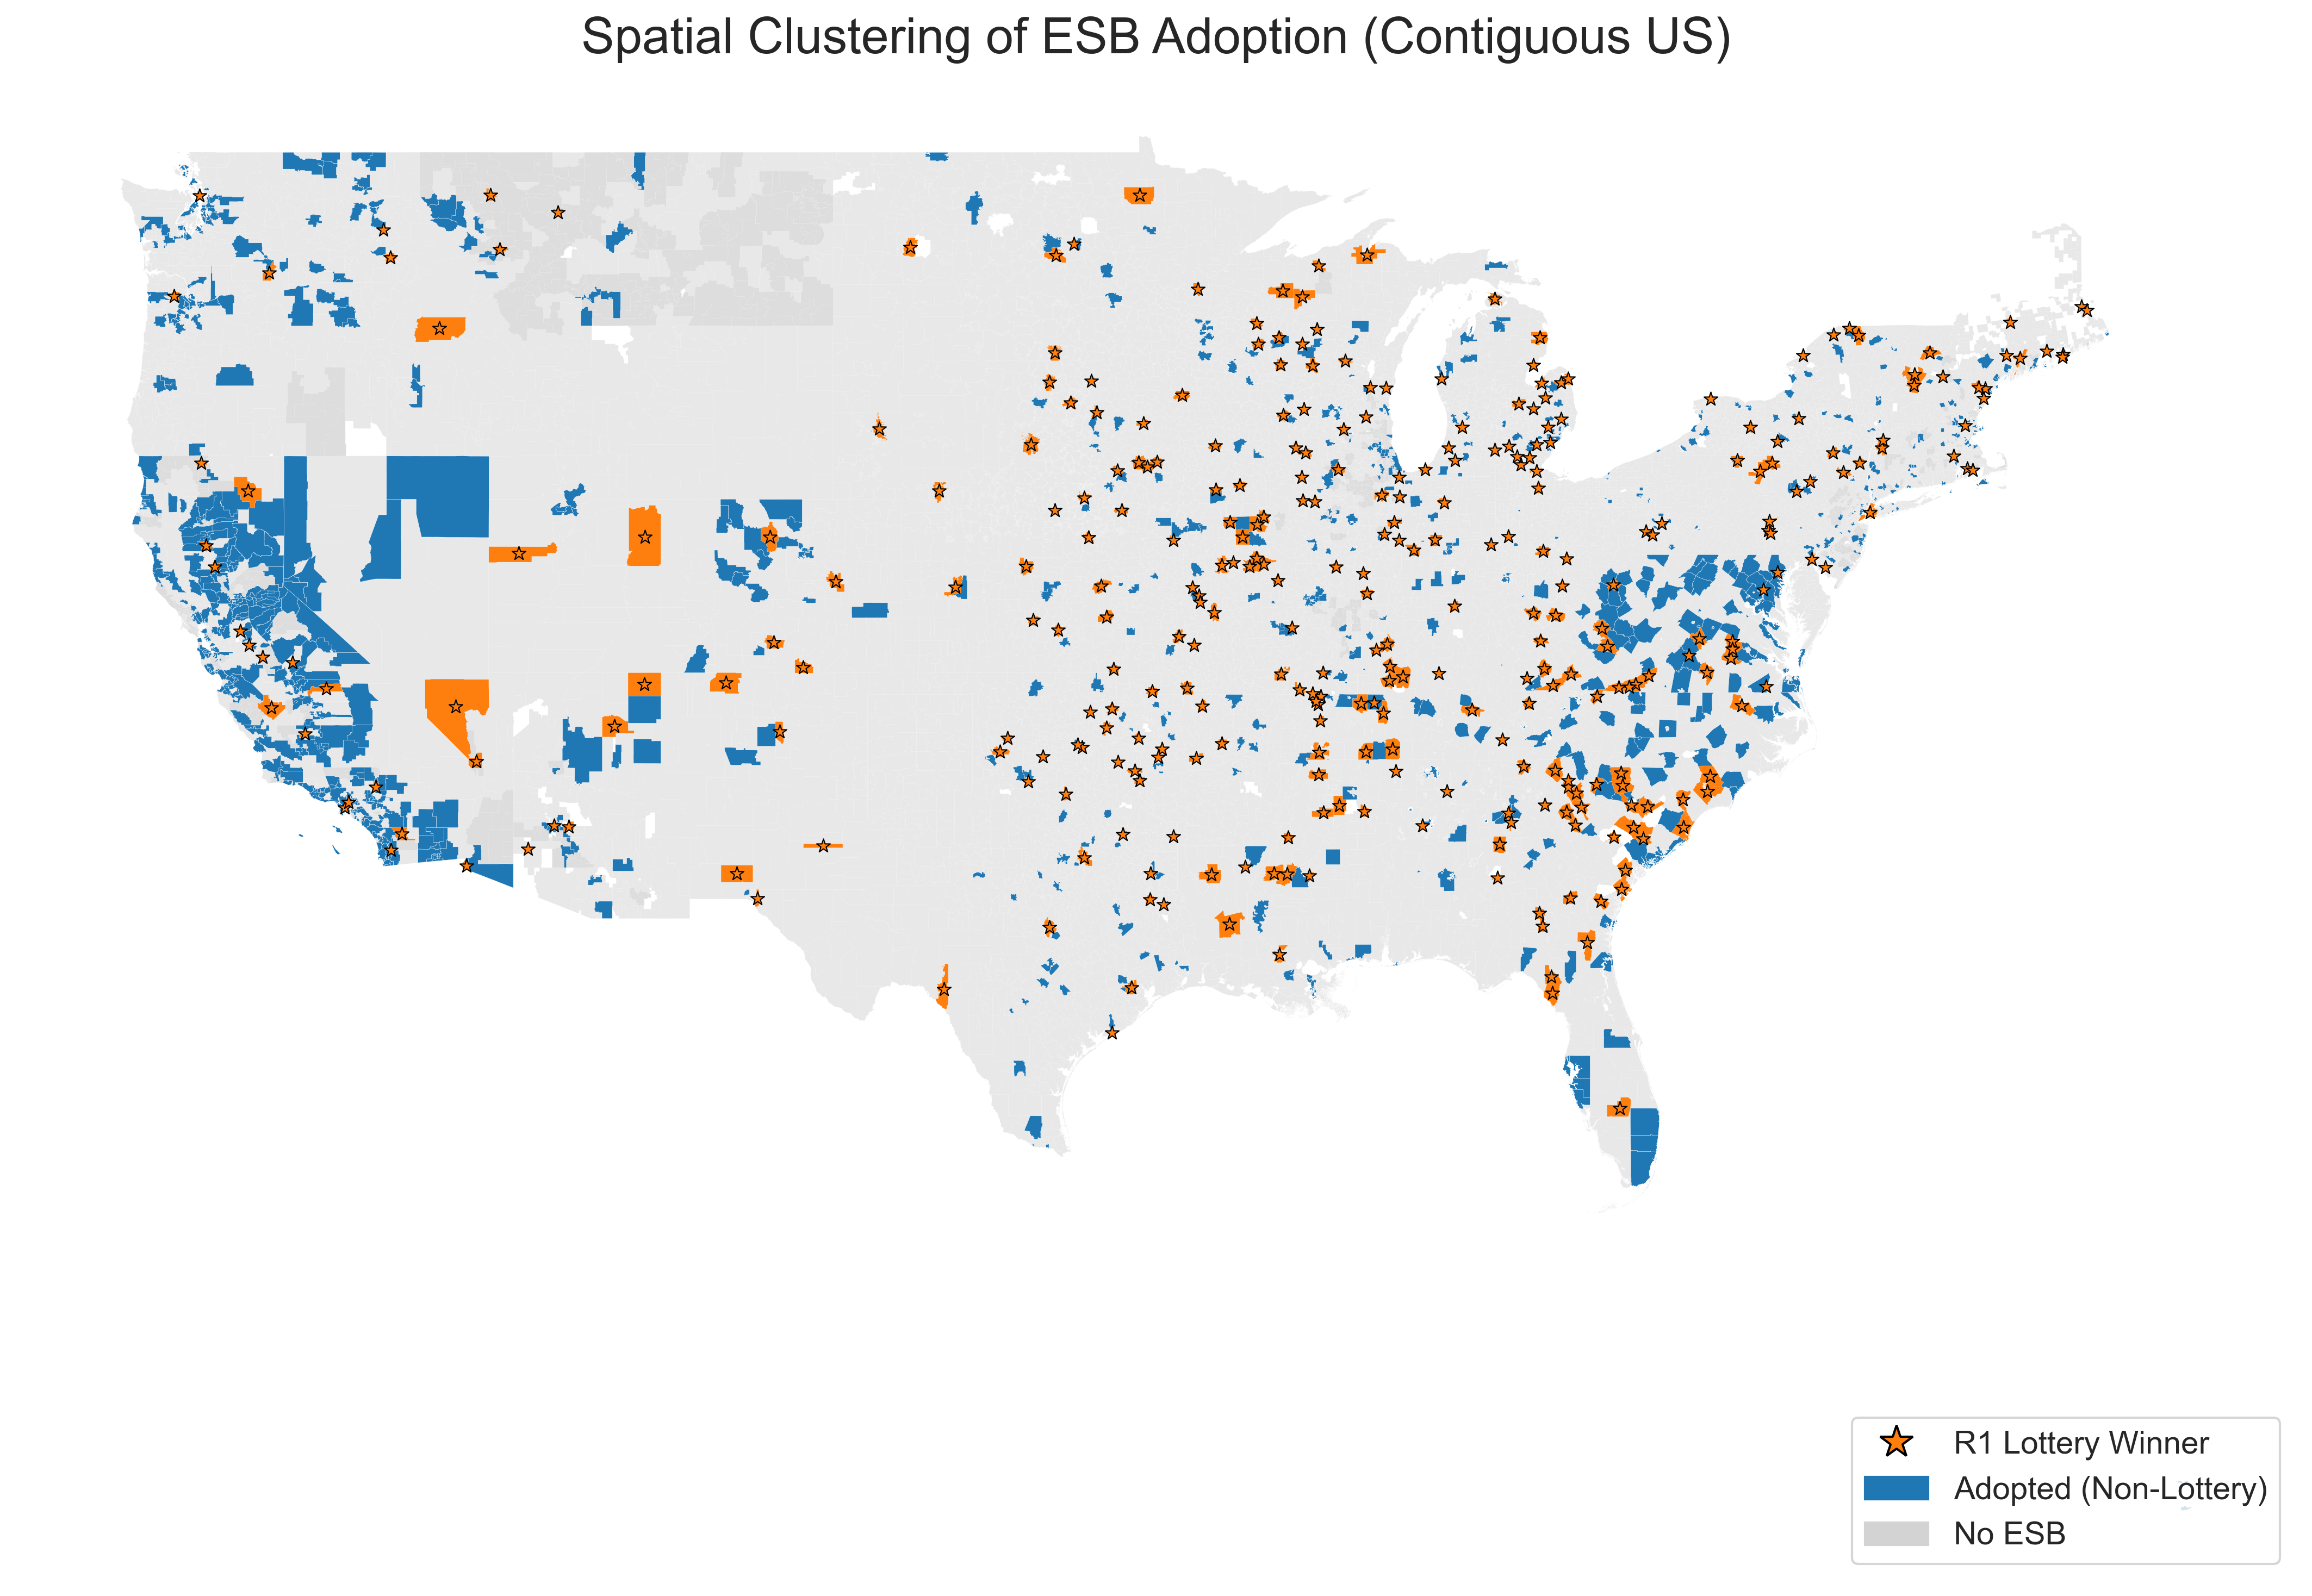
\includegraphics[width=0.85\textwidth]{esb_adoption_map_national.png}
\end{frame}

\begin{frame}{Descriptive Evidence: Raw Homophily}
    \centering
    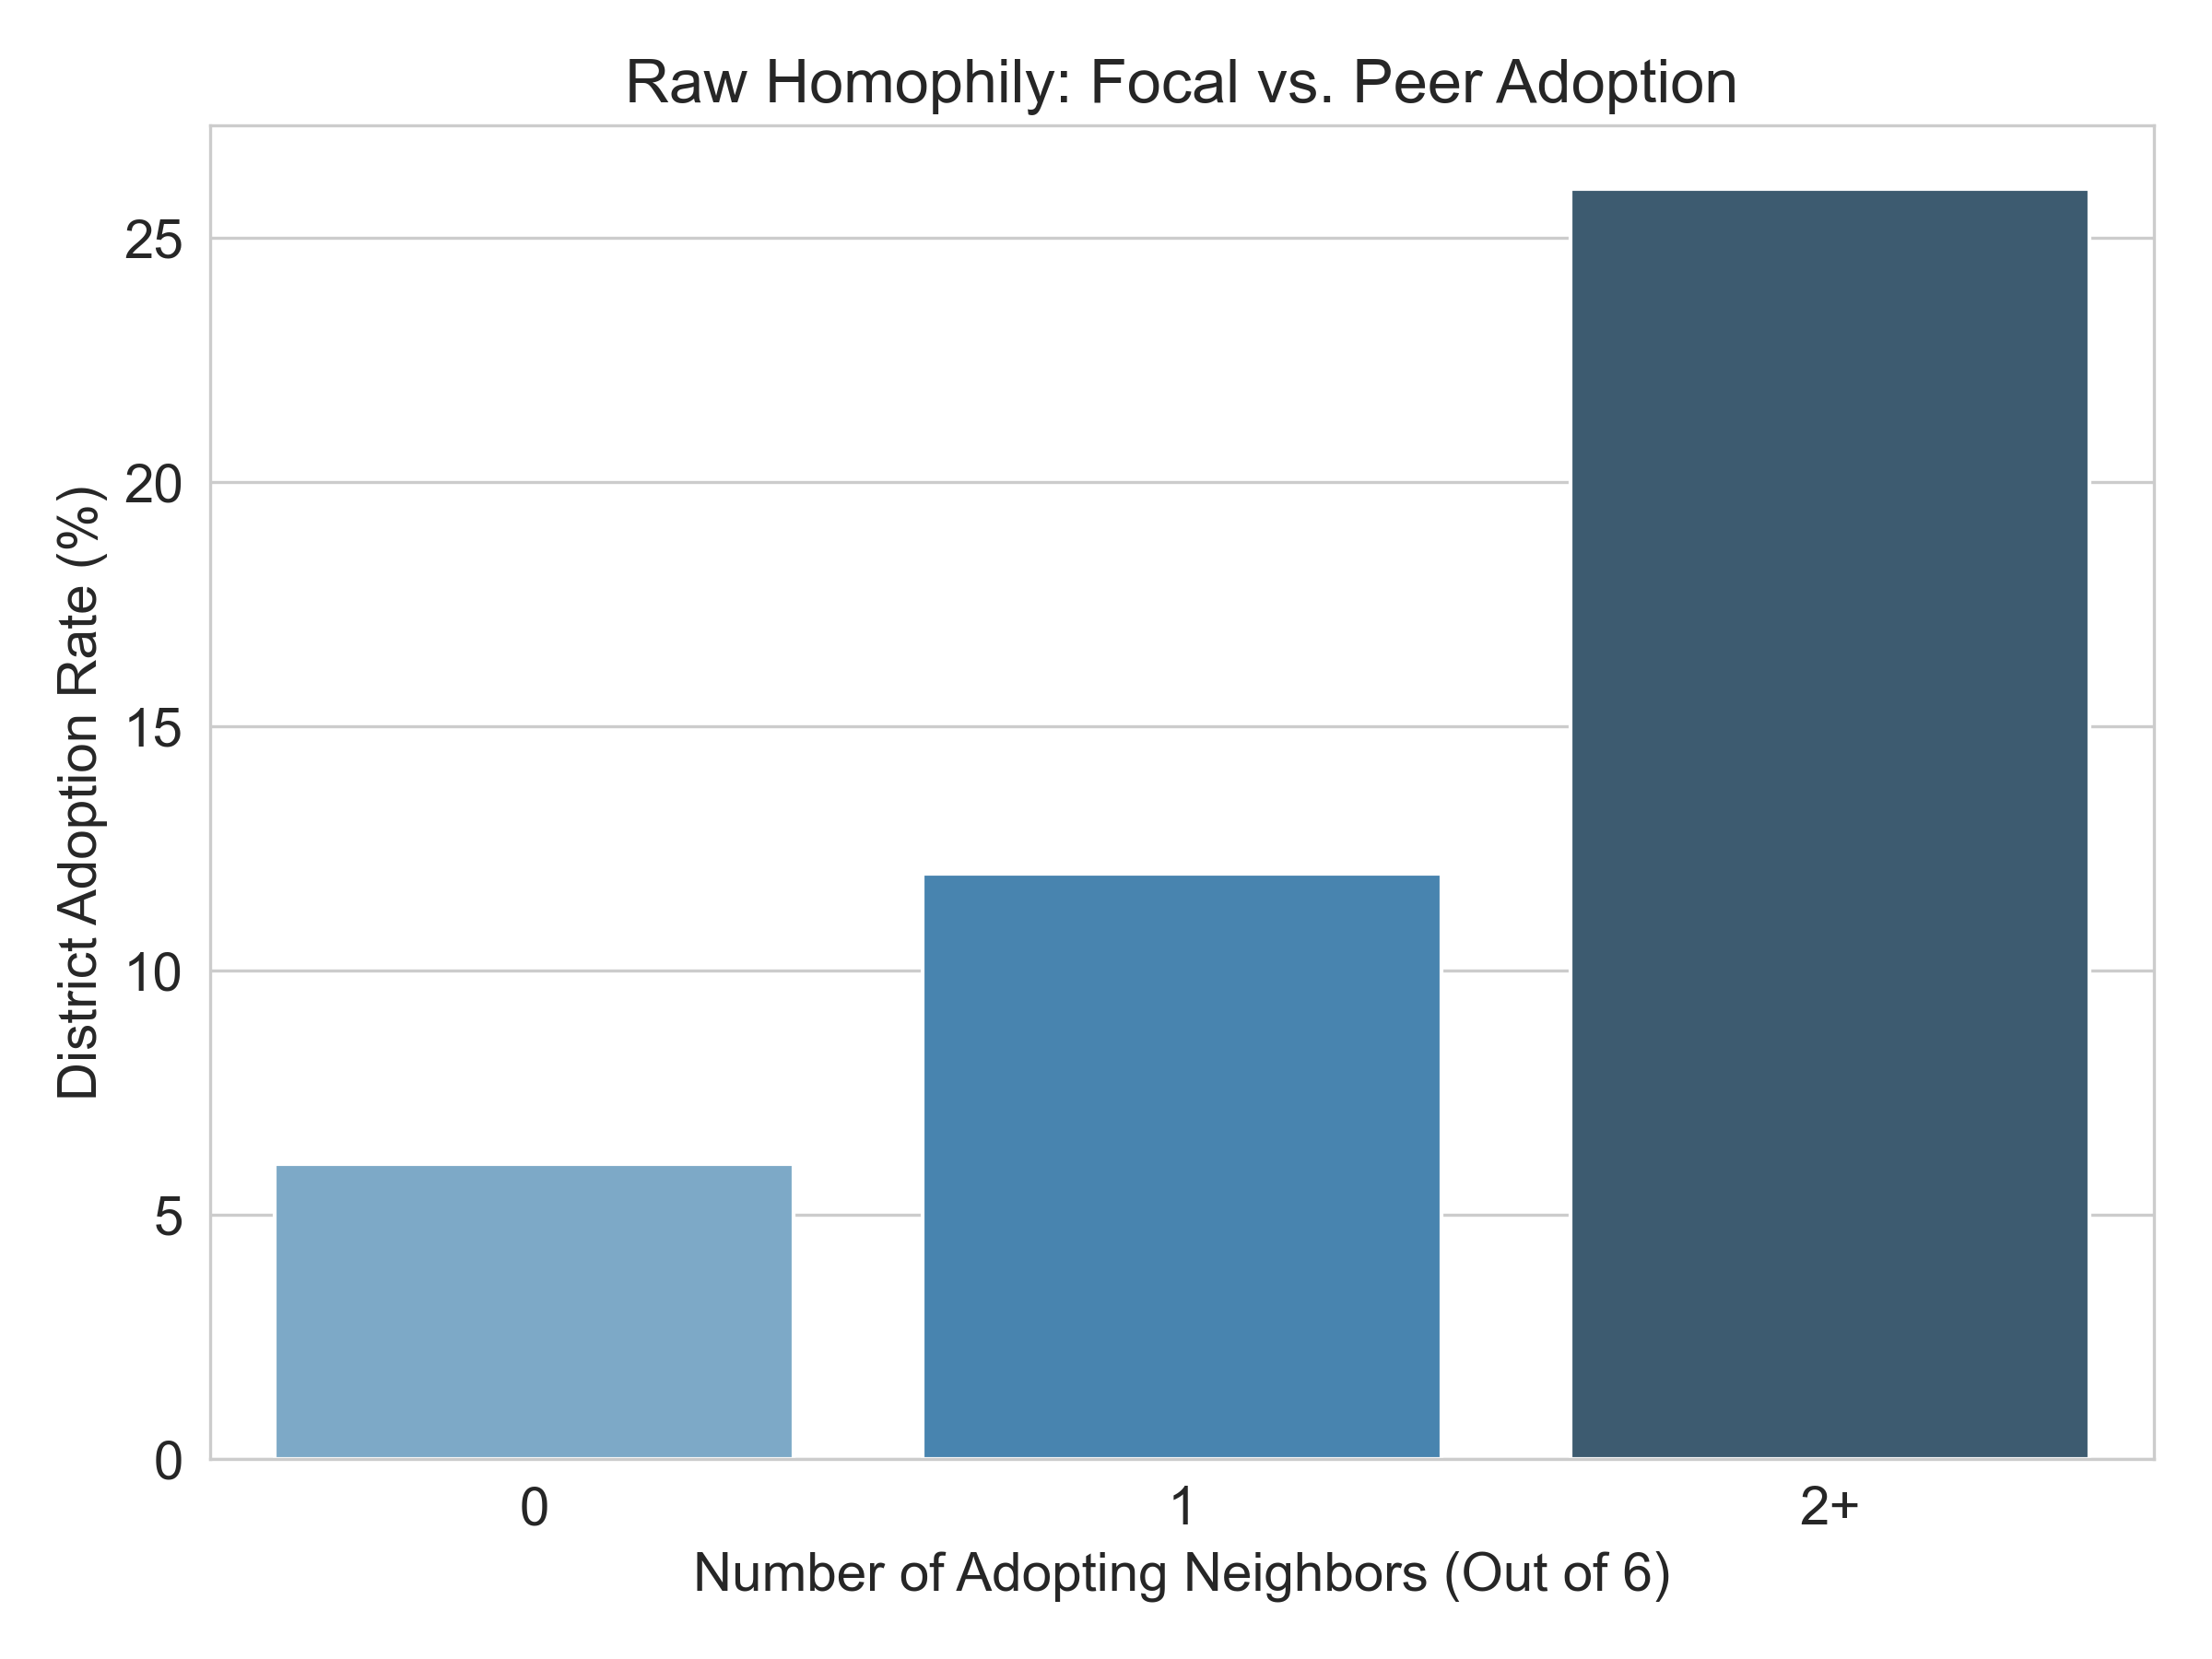
\includegraphics[width=0.7\textwidth]{naive_homophily_gradient.png}
    
    \begin{itemize}
        \item The raw gradient demonstrates high homophily: a district with 0 adopted neighbors adopts at 6.0\%, while a district with 2+ adopted neighbors adopts at 26.0\%.
        \item \textit{Challenge:} This reflects common unobservables just as much as learning. We need an identification strategy.
    \end{itemize}
\end{frame}

% -------------------------
% SECTION III: EMPIRICAL STRATEGY
% -------------------------

\begin{frame}{The Reflection Problem}
    \begin{itemize}
        \item A naive model regressing $Y_{i,t}$ on $P_{i,t-1}$ suffers from three severe biases:
        \begin{enumerate}
            \item \textbf{Simultaneity:} Focal district behavior affects peer behavior simultaneously.
            \item \textbf{Correlated Unobservables:} Shared state policies, infrastructure, or utility readiness.
            \item \textbf{Endogenous Network Formation:} Districts with similar preferences may geographically sort.
        \end{enumerate}
    \end{itemize}
\end{frame}

\begin{frame}{Identification: The EPA CSB R1 Lottery}
    \begin{itemize}
        \item \textbf{The Instrument (^{R1}$):} The number (or share) of a district's defined peers that won the FY2022 EPA CSB lottery.
        \item \textbf{Temporal Lag:} Model utilizes the \textit{lagged} stock of peer adoptions ($P_{i,t-1}$) to cleanly break simultaneity.
        \item \textbf{Relevance:} Neighboring lottery wins strongly predict actual neighbor bus deployment.
        \item \textbf{Exclusion Restriction:} The neighboring lottery win only affects the focal district through peer knowledge spillovers, conditional on priority strata and state fixed-effects.
    \end{itemize}
\end{frame}

\begin{frame}{Estimating Equations: First Stage \& Instrument}
    \textbf{First Stage (Predicting Peer Adoption):}
    $$ P_{i,t-1} = \pi_0 + \pi_1 \big(Z_i^{R1}\times \mathbf{1}_{2023}\big) + \pi_2 \big(Z_i^{R1}\times \mathbf{1}_{2024}\big) + \theta A_i^{R1} + \eta P_i^{preR1} + X_{it}'\rho + \mu_s + \tau_t + u_{it} $$
    
    \begin{itemize}
        \item \textbf{$P_{i,t-1}$}: Stock of previously awarded neighbors (Endogenous focal variable).
        \item \textbf{$Z_i^{R1}$}: Number of neighbors awarded in the R1 lottery. Interacted with post-lottery years (2023, 2024) to capture the timeline of the shock.
        \item \textbf{$A_i^{R1}$}: Application density (Winners + Waitlisted neighbors). Crucial for controlling for correlated "green" community preferences.
    \end{itemize}
\end{frame}

\begin{frame}{Estimating Equations: Second Stage}
    \textbf{Second Stage (Discrete Time Hazard):}
    $$ Y_{it} = \alpha + \beta \widehat{P}_{i,t-1} + \phi A_i^{R1} + X_{it}'\gamma + \delta P_i^{preR1} + \mu_s + \tau_t + \varepsilon_{it} $$
    
    \begin{itemize}
        \item \textbf{$Y_{it}$}: Focal district's likelihood of adopting an ESB in year $t$.
        \item \textbf{$\widehat{P}_{i,t-1}$}: Instrumented stock of peer adoptions. $\beta$ captures the causal peer effect.
        \item \textbf{$X_{it}$}: Controls including enrollment, demographics, PM2.5, and focal priority status.
        \item \textbf{$P_i^{preR1}$}: Baseline peer adoption prior to the R1 shock, isolating only incremental post-R1 exogenous variation in peer adoption.
    \end{itemize}
\end{frame}

\begin{frame}{Identifying Assumptions}
    \begin{itemize}
        \item \textbf{Threat 1: Correlated Tastes (Homophily):} Geographic clusters share unobserved "green" preferences, driving both R1 applications and subsequent adoption independently of learning.
        \item \textit{Defense:} Correlated tastes drive \textit{applications}, but the lottery drives \textit{wins}. Conditional on the number of neighbors that applied, how many actually won is random. This perfectly isolates the spillover of a funded award versus an unfunded waitlist.
        \vspace{0.2cm}
        \item \textbf{Threat 2: EPA Targeting (Exclusion Restriction):} The EPA targeted subsequent competitive grants (e.g., R2) to geographic areas near R1 winners.
        \item \textit{Defense:} State fixed effects absorb regional targeting, and our explicit event-study timing uniquely maps to peer administrative application cycles rather than standalone EPA deployments. R3 was also a randomized lottery, mitigating longitudinal targeting concerns.
    \end{itemize}
\end{frame}

% -------------------------
% SECTION IV: RESULTS & DISCUSSION
% -------------------------

\begin{frame}[label=main_results]{Main Results (2SLS Estimation)}
    \centering
    \footnotesize
    \begin{tabular}{lccc}
        \toprule
        & \textbf{(1) OLS} & \textbf{(2) 2SLS (No Controls)} & \textbf{(3) 2SLS (Controls)} \\
        \midrule
        Peer Adoption ($\widehat{P}_{i,t-1}$) & -0.0017   & 0.0105*** &  0.0075*** \\
                                        & (0.0031)  & (0.0022)  & (0.0017) \\
        R1 Applicant Neighbor Density   & 0.0005    &           & 0.0001     \\
                                        & (0.0005)  &           & (0.0006) \\        
        $\log(\text{Student Enrollment}_{it})$  & 0.0071*** &           & 0.0071*** \\
                                        & (0.0019)  &           & (0.0019) \\
        EPA Priority District Status ($t$) & 0.0054*** &           & 0.0055*** \\
                                        & (0.0012)  &           & (0.0012) \\
        \midrule
        State Fixed Effects             & Yes       & Yes       & Yes \\
        Year Fixed Effects              & Yes       & Yes       & Yes \\
        First Stage F-Statistic         &           &           & \textbf{534.9} \\
        Observations                    & 86,960    & 86,960    & 86,960 \\
        \bottomrule
    \end{tabular}
    
    \vspace{0.2cm}
    \raggedright
    \scriptsize \textit{Notes:} Standard errors clustered at the state level to account for spatial and political correlation. Column (3) explicitly controls for the number of neighboring applicants (R1 application density), strictly isolating the exogenous variation of randomized neighbor lottery \textit{wins} apart from correlated neighbor "green" tastes. * p<0.10, ** p<0.05, *** p<0.01.
\end{frame}

\begin{frame}{Estimating Equations: Dynamic Reduced Form}
    To validate parallel trends and map the exact timing of the spillover, we estimate the dynamic event study (reduced form):
    $$ Y_{it} = \alpha + \sum_{k \neq 2022} \lambda_k \big(Z_i^{R1} \times \mathbf{1}\{t=k\}\big) + \phi A_i^{R1} + X_{it}'\gamma  + \delta P_i^{preR1} + \mu_s + \tau_t + \varepsilon_{it} $$
    
    \begin{itemize}
        \item \textbf{$\lambda_k$}: The incremental effect on focal adoption probability of having an additional R1-winning neighbor in year $k$, relative to the base year (2022).
        \item \textbf{Parallel Trends Check}: We expect pre-treatment coefficients ($\lambda_{2020}$, $\lambda_{2021}$) to be 0, confirming our instrument is independent of prior localized adoption trends.
        \item \textbf{Timing}: The policy treatment naturally induces a lag. Neighbors win in 2022, focal districts build administrative knowledge/apply in 2023, and officially win an award in 2024.
    \end{itemize}
\end{frame}

\begin{frame}{Dynamic Event Study (Parallel Trends)}
    \centering
    
\includegraphics[width=0.6\textwidth]{reduced_form_event_study.png}
    
    \footnotesize \textit{Note: Spike perfectly aligns with the latency required to observe a 2022 peer win, prepare a complex 2023 application, and win a 2024 award.}
\end{frame}

\begin{frame}{Defense of Main Estimate: Geometric Decay of Peer Effects}
    \centering
    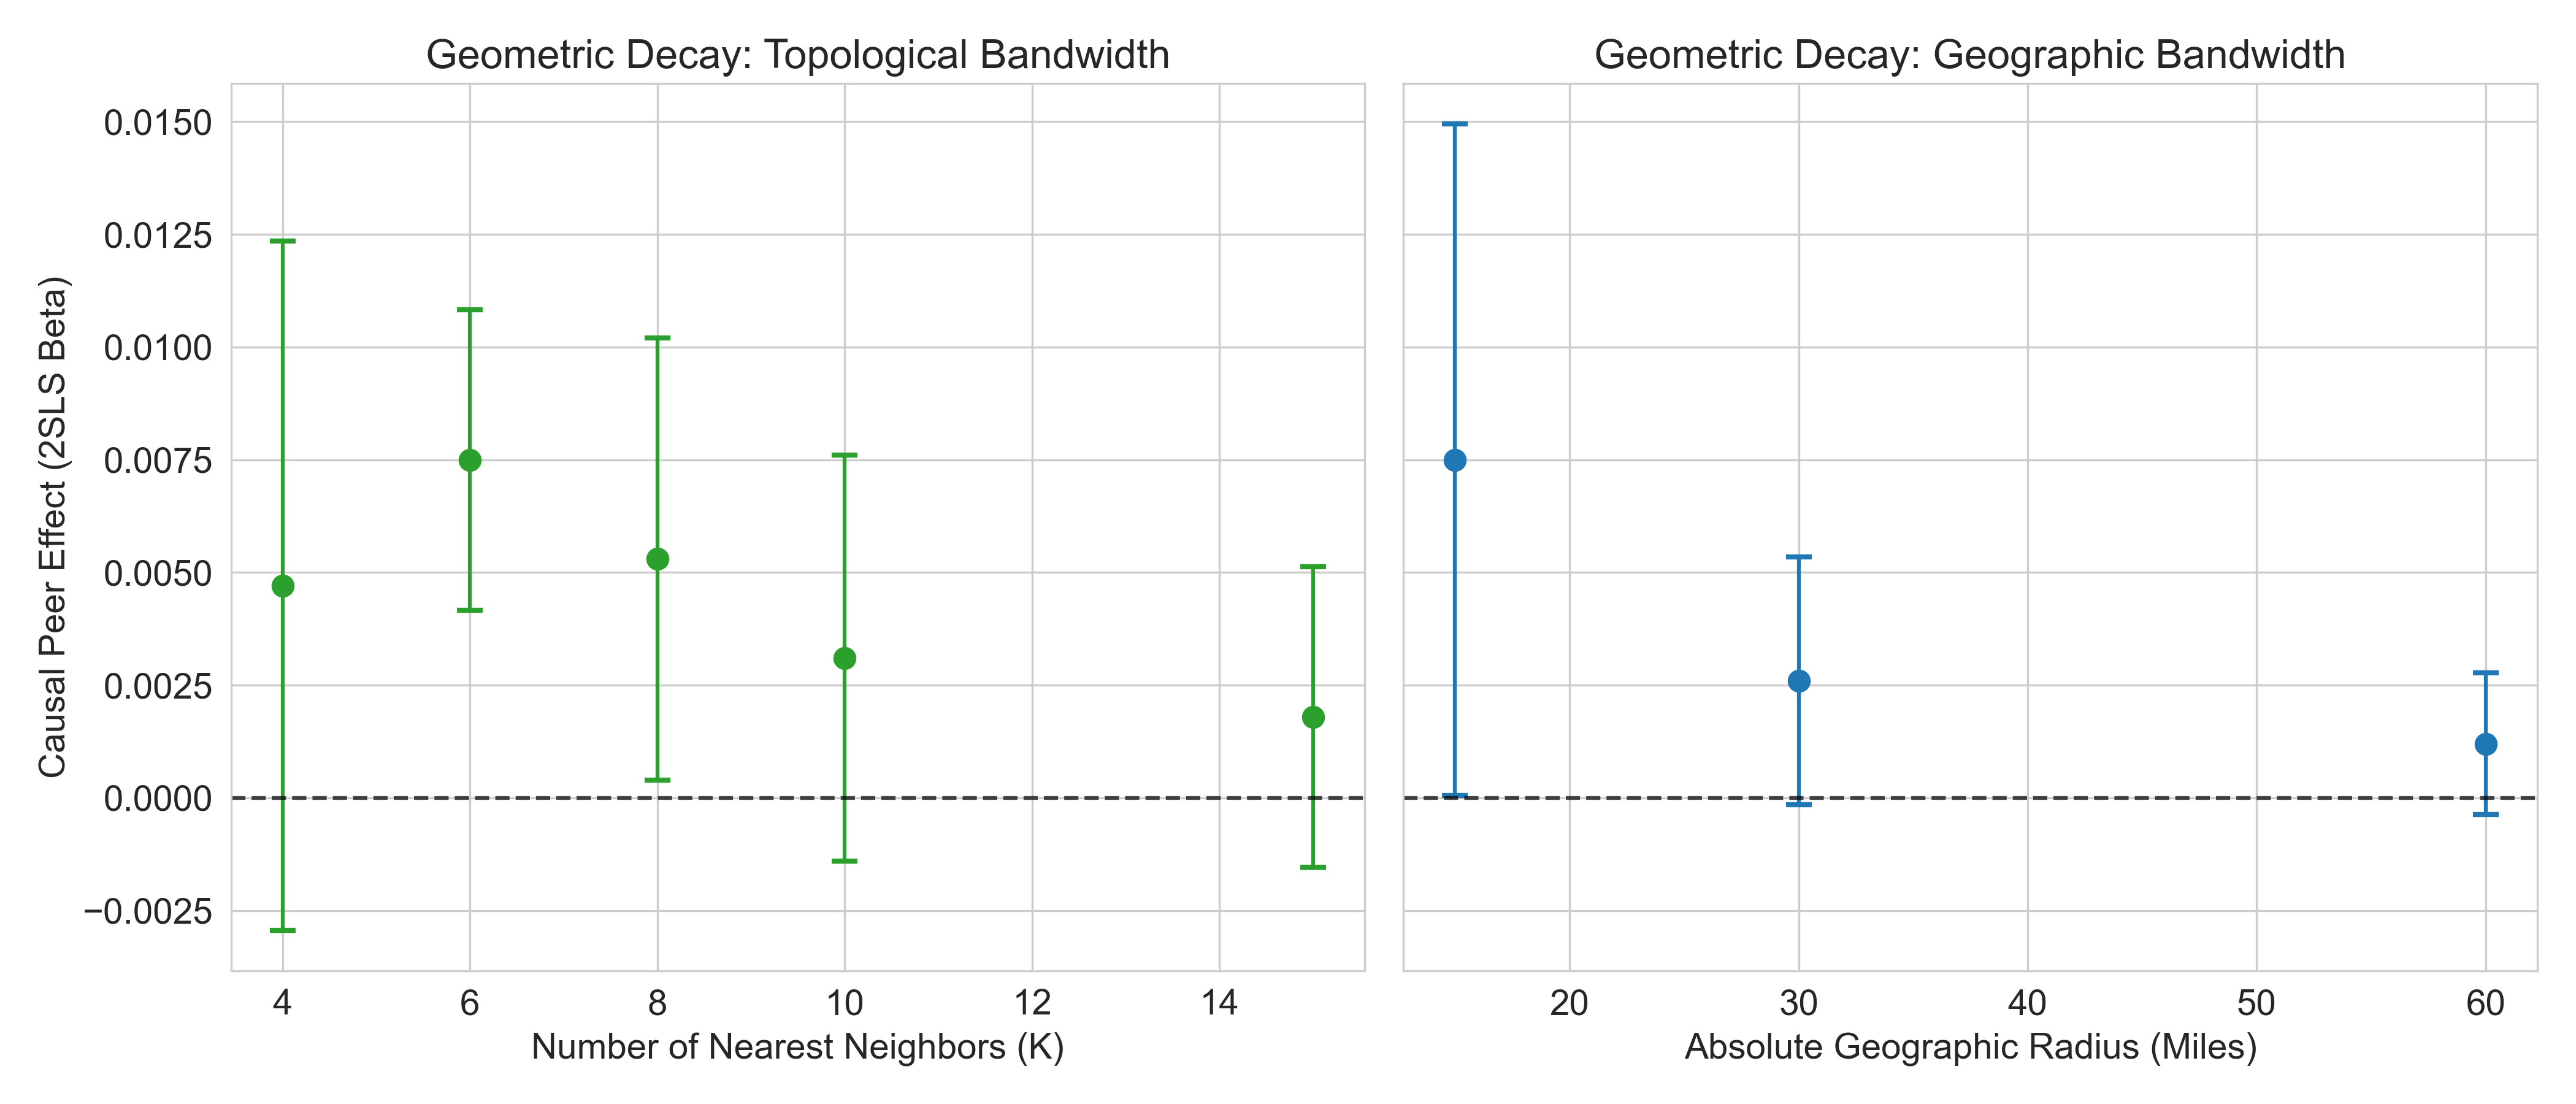
\includegraphics[width=0.85\textwidth]{spatial_decay_comparison.png}
\end{frame}

\begin{frame}{Geometric Decay Implications}
    \begin{itemize}
        \item The structural peer effect remains robust across topological measurements ($K \le 8$) and absolute geographic boundaries (15 Miles).
        \item \textbf{The Geometric Decay:} As we expand the radius outward (30 or 60 miles), the point estimate collapses back to zero.
        \item \textbf{Validation:} This monotonic spatial decay builds core confidence in the learning channel. True administrative knowledge transfer requires severe municipal proximity, unlike broader regional shocks.
    \end{itemize}
\end{frame}

\begin{frame}{Exploratory Mechanisms: Why does it cluster?}
    \begin{itemize}
        \item Are superintendents inspired by seeing a physical bus (Physical Salience), or by learning grant mechanics (Administrative Spillovers)?
        \item \textbf{Falsification Test:} There is a 12--18 month supply chain lag before a bus is delivered. We rerun the 2SLS model redefining adoption as the \textit{First Operating Year} (physical arrival).
        \vspace{0.3cm}
        \item \textbf{First Awarded IV Estimate:} $\beta = 0.0075^{***} \quad (SE = 0.0017)$
        \item \textbf{First Operating IV Estimate:} $\beta = -0.0005 \quad (SE = 0.0013)$
        \vspace{0.3cm}
        \item Suggestive evidence points directly toward administrative capacity and application-coordination over physical visibility.
    \end{itemize}
\end{frame}

\begin{frame}{Preliminary Policy Implications}
    \begin{itemize}
        \item Federal infrastructure programs may not be merely zero-sum payouts; they can generate meaningful administrative network effects.
        \item \textbf{The localized multiplier:} Suggestive evidence indicates a single grant acts as a localized capacity-building shock for neighboring applications.
        \item \textbf{Target formulation (WIP):} If the goal is rapid EV transition, granting agencies might consider the spillover value of subsidizing key density nodes to catalyze voluntary peripheral adoption, without triggering additional standalone EPA grant funding needs everywhere.
    \end{itemize}
\end{frame}

% -------------------------
% SECTION V: CONCLUSION
% -------------------------

\begin{frame}{Next Steps \& Takeaways}
    \begin{itemize}
        \item \textbf{Current Takeaways:} District-level adoption of Electric School Buses demonstrates robust localized peer effects. By instrumenting with randomized EPA CSB R1 lotteries, we isolate unobserved homophily.
        \item \textbf{Mechanism Insight:} The 12-to-18-month latency implies administrative capacity spillovers over physical salience. Severe spatial bounding (<15mi) confirms network intensity requirements.
        \item \textbf{Next Steps for the Project:} 
        \begin{itemize}
            \item Formalize robustness bounds for remaining unobservables.
            \item Expand mechanism investigations by parsing identical bus vendors or shared consulting firms.
            \item Formalize comprehensive balance testing across spatial definitions.
        \end{itemize}
    \end{itemize}
\end{frame}

\appendix
\begin{frame}[label=app_summary]{Appendix A: Basic Sample Descriptives}
    \centering
    \begin{table}
        \small
        \begin{tabular}{lccccc}
            \toprule
            \textbf{Metric} & \textbf{Universe} & \textbf{Estimation} & \textbf{Adopters} & \textbf{Non-Adopters} & \textbf{P-value} \\
            \midrule
            Count ($n$) & 19,495 & 12,694 & 1,536 & 17,959 & -- \\
            Adoption Rate & 7.9\% & 8.2\% & 100\% & 0\% & -- \\
            Mean Enrollment & 2,685 & 3,413 & 10,292 & 2,013 & <0.001 \\
            Median Enrollment & 702 & 1,098 & 2,691 & 644 & -- \\
            Mean Income (\$) & 69,026 & 69,375 & 68,874 & 69,043 & <0.001 \\
            Mean Poverty Rate & 12.2\% & 12.0\% & 13.8\% & 11.9\% & <0.001 \\
            Mean \% White & 82.1\% & 82.2\% & 72.6\% & 83.2\% & <0.001 \\ 
            Mean PM2.5 ($\mu g/m^3$) & 7.34 & 7.36 & 7.56 & 7.31 & <0.001 \\
            \midrule
            \multicolumn{6}{l}{\textbf{Urbanicity Distribution}} \\
            Rural & 42.1\% & 53.0\% & 35.6\% & 42.6\% & 0.038 \\
            Suburban & 23.2\% & 23.4\% & 26.3\% & 22.9\% & 0.367 \\
            Town & 15.6\% & 18.0\% & 14.8\% & 15.7\% & 0.609 \\
            Urban & 19.1\% & 5.6\% & 22.7\% & 18.8\% & 0.226 \\
            \bottomrule
        \end{tabular}
    \end{table}
    \vspace{0.2cm}
    \hyperlink{summary_balance}{\textbf{\color{mLightBrown} $\leftarrow$ Back to Main}}
\end{frame}

\begin{frame}[label=app_balance]{Appendix B: Pre-R1 Group Balance (Priority Applicant Pool)}
    \centering
    \begin{table}
        \footnotesize
        \begin{tabular}{lcccc}
            \toprule
            \textbf{Observable Characteristic} & \textbf{Winner Mean} & \textbf{Loser Mean} & \textbf{Difference} & \textbf{P-value} \\
            \midrule
            Enrollment & 6,877 & 4,136 & 2,741 & 0.068 \\
            Median Income (\$) & 55,815 & 55,258 & 556 & 0.560 \\
            Poverty Rate & 15.9\% & 16.1\% & -0.2\% & 0.700 \\
            \% White Demographic & 78.1\% & 78.9\% & -0.8\% & 0.564 \\
            Baseline PM2.5 ($\mu g/m^3$) & 7.42 & 7.40 & 0.02 & 0.811 \\
            Pre-2022 Early Adopter & 3.1\% & 3.2\% & -0.1\% & 0.973 \\
            \bottomrule
        \end{tabular}
    \end{table}
    \vspace{0.2cm}
    \hyperlink{summary_balance}{\textbf{\color{mLightBrown} $\leftarrow$ Back to Main}}
\end{frame}

\end{document}
